\chapter{Galois Fields Preliminaries and Application in Hardware Design} \label{ch:prelim}
This chapter provides a mathematical background for understanding 
Galois fields and explains how to design Galois field arithmetic circuits.
We first introduce the mathematical concepts of groups, rings, fields, and 
polynomials. 
We then apply these concepts to create Galois field arithmetic functions and 
explain how to map them to a Boolean circuit implementation.
The material is referred from \cite{galois_field:mceliece} \cite{ftheory:2006} \cite{ff:1997} for Galois field concepts and 
\cite{mastro:1989} \cite{PT:1985} \cite{acar:1998} \cite{wu:2002} \cite{Knezevic:2008} for hardware design over Galois fields and previous work
by {\it Lv} \cite{lv:phd}.

%%%%%%%%%%%%%%%%%%%%%%%%%%%%%%%%%%%%%%%%%%%%%%%%%%%%%%%%%%%%%%%%%%%%%%%%%%%%%%%

\section{Rings, Fields and Polynomials}

\begin{Definition}
An {\bf abelian group} is a set $\mathbb{S}$ with a binary operation $'+'$
which satisfies the following properties: 
\begin{itemize}
\item {\it Closure Law:} For every $a, b \in \mathbb{S}, a + b \in \mathbb{S}$  
\item {\it Associative Law:} For every $a, b, c \in \mathbb{S}, (a + b) + c = a + (b + c)$
\item {\it Commutativity:} For every $a, b \in \mathbb{S}, a + b = b + a$. 
\item {\it Additive Identity:} There is an identity element $0 \in \mathbb{S}$
such that for all $a \in \mathbb{S};$ $a + 0 = a$.
\item {\it Additive Inverse:} If $a \in \mathbb{S}$, then there is an
element $a^{-1} \in \mathbb{S}$ such that $ a + a^{-1} = 0$.
\end{itemize}
\end{Definition}

The set of integers $\mathbb{Z}$ forms an abelian group under the addition operation. 

\begin{Definition}
Given a set $\mathbb{R}$ with two binary operations, $'+'$ and $'\cdot'$, 
and element $0 \in \mathbb{R}$, the system $\mathbb{R}$ is called a {\bf commutative ring with unity} if the following properties hold:
\begin{itemize}
\item $\mathbb{R}$ forms an abelian group under the '+' operation with additive identity element $0$.
\item {\it Multiplicative Distributive Law}: For all $a, b, c \in$ $\mathbb{R}$, $a\cdot (b + c) = a\cdot b + a\cdot c$.
\item {\it Multiplicative Associative Law}: For every $a, b, c\in \mathbb{R}$, $a\cdot (b\cdot c) = (a\cdot b)\cdot c$. 
\item {\it Multiplicative Commutative Law}: For every $a,b \in \mathbb{R}$, $a\cdot b = b\cdot a$
\item {\it Identity Element}: There exists an element $1 \in$ $\mathbb{R}$ 
such that for all $a \in \mathbb{R}$, $a\cdot 1 = a =1\cdot a$
\end{itemize}
\end{Definition}

For the purpose of this dissertation, any time we refer to a {\bf ring}, we are 
specifically referring to a {\bf commutative ring with unity}. Two common 
examples of such rings are the set of integers, $\mathbb{Z}$, and the set of 
rational numbers, $\mathbb{Q}$. Note that while both of these examples are
rings with an infinite number of elements, the number of elements in a ring 
can also be finite.

\begin{Definition}
The {\bf modular number system} with base $n$ is a set of positive
integers $Z_n = \{0, 1, \ldots, n-1\}$, with the two operations $+$
and $\cdot$ satisfying the properties below:
\begin{eqnarray}
(a + b)\pmod{ n } &\equiv& ((a ~\pmod {n}) + (b ~\pmod {n})) ~\pmod {n} \nonumber\\
(a\cdot b) ~\pmod {n} &\equiv& ((a ~\pmod {n}) \cdot (b ~\pmod {n})) ~\pmod {n} \label{eq:modmult}\nonumber\\
(-a) ~\pmod {n} &\equiv& (n-a) ~\pmod {n}\nonumber 
\end{eqnarray}
\end{Definition}


\begin{Example}
The set $Z_8 = \{0, 1, \ldots, 7\}$ denotes the modular number system
with base $8$. Examples of some operations performed $\pmod {8}$
are:
\begin{eqnarray} \nonumber
        3 + 6   &~=& 9  ~\pmod{8} ~= 1 \nonumber \\
        3 \cdot 6   &~=& 18 ~\pmod{8} ~= 2 \nonumber \\
        (-3)    &~=& 8-3  ~\pmod{8} ~= 5 \nonumber
\end{eqnarray} \nonumber
\end{Example}

The modular number system $\mathbb{Z}_n = \{0, 1, \ldots, n-1\}$, where $n$ 
is a positive integer, forms a ring.
Since this type of ring contains a finite number of elements $n$,
it is termed a {\it finite integer ring}, where addition and multiplication 
are computed {\it modulo n} $\pmod {n}$. 
In hardware applications, arithmetic over $k$-bit vectors manifests itself 
as algebra over the finite integer ring $\mathbb{Z}_{2^k}$, where the $k$-
bit vector represents integer values from $\{0, ...., 2^k-1\}$.

\begin{Example}
\label{exp:4bitadder}
Consider the following arithmetic circuit:

\begin{figure}[!h]
\centerline{
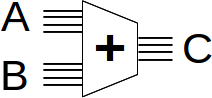
\includegraphics[width=0.3\textwidth]{figures/4bitMultTop}
}
%\caption{Typical hardware design flow.}
%\label{fig:cadflow}
\end{figure}

This circuit takes two 4-bit inputs, $A$ and $B$, and computes a 4-bit sum $C$. 
Since $A$, $B$, and $C$ are all bit-vectors of size $4$, 
the addition computation this circuit performs is modulo $2^4$.
Hence, this circuit exemplifies arithmetic computations over the ring $Z_{2^4}$.

Some examples of possible inputs and outputs of the circuit:
\begin{table}[!h]
	\centering
	\begin{tabular}{|lll|lll|}
	\hline
	\multicolumn{3}{|c|}{Addition over $\mathbb{Z}_{2^4}$} & \multicolumn{3}{c|}{Boolean Circuit Implementation} \\
	\hline
	$5 + 8$ & $~=$ & $13 ~\pmod{16} ~= 13$ & $A=0101$, $B=1000$ & $\rightarrow$ &  $C=1101$ \\
	$10 + 9$ & $~=$ & $ 19 ~\pmod{16} ~= 3$ & $A=1010$, $B=1001$ & $\rightarrow$ &  $C=0011$ \\
	$12 + 4$ & $~=$ & $ 16 ~\pmod{16} ~= 0$ & $A=1100$, $B=0100$ & $\rightarrow$ &  $C=0000$ \\
	\hline
	\end{tabular}
\end{table}
\end{Example}

\begin{Definition}\label{def:poly}
Let $\mathbb{R}$ be a ring. A {\bf polynomial} over $\mathbb{R}$ in the 
indeterminate $x$ is an expression of the form:
\begin{equation} \label{eq:poly1}
a_0 + a_1 x + a_2 x^2 + \cdots + a_k x^k = \sum_{i=0}^{k} a_i x^i, \forall a_i \in \mathbb{R}. 
\end{equation}

\end{Definition}

The constants $a_i$ are the coefficients and $k$ is the degree of the polynomial. 
For example, $8x^3 + 6x + 1$ is a polynomial in $x$ over $\mathbb{Z}$, with
coefficients $8$, $6$, and $1$ and degree $3$. 

\begin{Definition}
The set of all polynomials in the indeterminate
$x$ with coefficients in the ring $\mathbb{R}$ forms a {\bf
ring of polynomials} $\mathbb{R}[x]$. 
Similarly, $\mathbb{R}[x_1,x_{2},\cdots, x_{n}]$ 
represents the ring of multivariate polynomials with coefficients in $\mathbb{R}$.
\end{Definition}

For example, $\mathbb{Z}_{2^4}[x]$ stands for the set of all polynomials in
$x$ with coefficients in $\mathbb{Z}_{2^4}$. $8x^3 + 6x + 1$ is an instance 
of a polynomial contained in $\mathbb{Z}_{2^4}[x]$.

\begin{Definition}
A {\bf field} $\mathbb{F}$ is a commutative ring with unity, where every
non-zero element in $\mathbb{F}$ has a multiplicative inverse; i.e. $\forall
a \in \mathbb{F} - \{0\}$, $\exists \hat{a} \in \mathbb{F}$ such that $ a \cdot
\hat{a} = 1$.
\end{Definition}

A field is defined as a ring with one extra condition: the presence of a 
multiplicative inverse for all non-zero elements.
Therefore, a field must be a ring while a ring is not necessarily a field.
For example, the set $\mathbb{Z}_{2^k} = \{0,1,\cdots, 2^k-1\}$ forms a finite ring.
However, $\mathbb{Z}_{2^k}$ is not a field because not every element in
$\mathbb{Z}_{2^k}$ has a multiplicative inverse. 
In the ring $\mathbb{Z}_{2^3}$, for 
instance, the element $5$ has an inverse ($5\cdot5\pmod{8}=1$) but the element $4$
does not.

The main concept of field theory is {\bf Field Extensions}. The idea behind a
field extension is to take a base field and construct a larger field which 
contains the base field as well as satisfies additional properties. For example,
the set of real numbers $\mathbb{R}$ forms a field; one common extension of 
$\mathbb{R}$ is the set of complex numbers $\mathbb{C}=\mathbb{R}(i)$. Every
element of $\mathbb{C}$ can be represented as $a+b\cdot i$ where $a,b \in \mathbb{R}$,
hence $\mathbb{C}$ is a two-dimensional extension of $\mathbb{R}$.

Like rings, fields can also contain either an infinite or a finite number of 
elements. 
In this dissertation we focus on finite fields, also known as Galois fields, and 
the construction of their field extensions.

%%%%%%%%%%%%%%%%%%%%%%%%%%%%%%%%%%%%%%%%%%%%%%%%%%%%%%%%%%%%%%%%%%%%%%%%%%%%
%%%%%%%%%%%%%%%%%%%%%%%%%%%%%%%%%%%%%%%%%%%%%%%%%%%%%%%%%%%%%%%%%%%%%%%%%%%%
%%%%%%%%%%%%%%%%%%%%%%%%%%%%%%%%%%%%%%%%%%%%%%%%%%%%%%%%%%%%%%%%%%%%%%%%%%%%%
\section{Galois Fields}\label{sec:ff}
Galois fields, also known as finite fields, find widespread applications in 
many areas of electrical engineering and computer science such as error-
correcting codes, elliptic curve cryptography, digital signal processing, 
testing of VLSI circuits, among others.
In this dissertation, we specifically focus on their application to 
Elliptic Curve Cryptography as Galois field arithmetic circuits.
This section describes the relevant Galois field concepts
\cite{galois_field:mceliece} \cite{ftheory:2006} \cite{ff:1997}
and hardware arithmetic designs over such fields \cite{mastro:1989} \cite{PT:1985} 
\cite{acar:1998} \cite{wu:2002} \cite{Knezevic:2008}. 

%%%%%%%%%%%%%%%%%%%%%%%%%%%%%%%%%%%%%%%%%%%%%%%%%%%%%%%%%%%%%%%%%%%%%%%%%%%%

\begin{Definition} 
A {\bf Galois field}, denote $\Fq$, is a field with a finite
number of elements, $q$. The number of elements $q$ of the Galois field is
a power of a prime integer, i.e. $q = p^k$, where $p$ is a prime
integer, and $k \geq 1$. Thus a Galois field can also be denoted as 
$\F_{p^{k}}$.
\end{Definition}

Fields in the form $\F_{p^{k}}$ are called Galois extension fields.
We are specifically interested in extension fields of type 
$\Fkk$, where $k > 1$. These are extensions of the binary
field $\F_2$.
\begin{Example}
Addition and multiplication operations over $\F_2$:
\begin{table}[!h]
	\centering
	\begin{tabular}{m{1cm}|l|ll|m{1cm}}
	\hhline{~---~}
	\multirow{3}{*}{} & $+$ & $0$ & $1$ & \multirow{3}{*}{} \\
	\hhline{~---~}
	& $0$ & $0$ & $1$ & \\
	& $1$ & $1$ & $0$ & \\
	\hhline{~---~}
	\multicolumn{5}{c}{}\\
	\multicolumn{5}{c}{Addition over $\F_2$}\\
	\end{tabular}
	\quad
	\begin{tabular}{m{1cm}|l|ll|m{1cm}}
	\hhline{~---~}
	\multirow{3}{*}{} & $\cdot$ & $0$ & $1$ & \multirow{3}{*}{} \\
	\hhline{~---~}
	& $0$ & $0$ & $0$ & \\
	& $1$ & $0$ & $1$ & \\
	\hhline{~---~}
	\multicolumn{5}{c}{}\\
	\multicolumn{5}{c}{Multiplication over $\F_2$}\\
	\end{tabular}
\end{table}

Notice that addition over $\F_2$ is a Boolean {\sc XOR} operation, 
because it is performed modulo $2$.
Similarly, multiplication over $\F_2$ performs a Boolean {\sc AND} operation.
\end{Example}

Algebraic extensions of the binary field $\F_{2}$  
are generally termed as {\it binary extension fields} $\Fkk$.
Where elements in $\F_2$ can only represent $1$ bit, elements in $\Fkk$ 
represent a $k$-bit vector.
This allows them to be widely used in digital hardware applications.
In order to construct a Galois field of the form $\Fkk$, 
an {\bf irreducible polynomial} is required:
\begin{Definition}
A polynomial $P(x) \in \mathbb{F}_{2}\left[x\right]$ is {\bf irreducible} 
if $P(x)$ is non-constant with degree $k$ and cannot be 
factored into a product of polynomials of lower degree in $\mathbb{F}_2[x]$.
\end{Definition}

Therefore, the polynomial $P(x)$ with degree $k$ is irreducible over 
$\mathbb{F}_{2}$ if and only if it has no roots in $\mathbb{F}_{2}$,
i.e if $\forall a \in \mathbb{F}_{2}$, $P(a)\neq 0$.
For example, $x^2+x+1$ is an irreducible polynomial over $\mathbb{F}_{2}$
because it has no solutions in $\mathbb{F}_{2}$, i.e. $(0)^2+(0)+1=1\neq0$ 
and $(1)^2+(1)+1=1\neq0$ over $\F_2$.
Irreducible polynomials exist for any degree $\geq 2$ in $\mathbb{F}_2[x]$.

Given an irreducible polynomial $P(x)$ of degree $k$ in the polynomial ring 
$\mathbb{F}_2[x]$, we can construct a binary extension field 
$\mathbb{F}_{2^k} \equiv \mathbb{F}_2[x] \pmod{P(x)}$.
Let $\alpha$ be a root of $P(x)$, i.e., $P(\alpha)=0$.
Since $P(x)$ is irreducible over
$\mathbb{F}_2[x]$, $\alpha \notin \mathbb{F}_2$. 
Instead, $\alpha$ is an element in $\mathbb{F}_{2^k}$. 
Any element $A \in \mathbb{F}_{2^k}$ is then represented as: 
\begin{equation}\label{rep:poly}
A= \sum_{i=0}^{k-1} (a_i \cdot \alpha^i) = a_0 + a_1\cdot\alpha + \cdots + a_{k-1}\cdot \alpha^{k-1}\nonumber
\end{equation}
where $a_i \in \mathbb{F}_2$ are the coefficients and $P(\alpha)=0$.

To better understand this field extension, compare its similarities to another
common-place
field extension $\C$, the set of complex numbers. $\C$ is an extension of the field 
of real numbers $\R$ with an additional element $i=\sqrt{-1}$, which is an imaginary
root in $\R$.
Thus $i \notin \R$, rather $i \in \C$.
Every element $A \in \mathbb{C}$ can be represented as:
\begin{equation}\label{rep:polyC}
A=\sum_{j=0}^{1} (a_j \cdot i^j)=a_0+a_1\cdot i
\end{equation}
where $a_j \in \R$ are coefficients. Similarly, $\Fkk$ is an extension of $\F_2$ with 
an additional element $\alpha$, which is the ``imaginary root'' of an irreducible 
polynomial $P$ in $\F_2[x]$.

Every element $A \in \Fkk$ has a degree less than $k$ because 
$A$ is always computed modulo $P(x)$, which has degree $k$. 
Thus, $A\pmod {P(x)}$ can be of degree at most $k-1$ and at least $0$.
For this reason, the field $\mathbb{F}_{2^k}$ can be viewed as a $k$
dimensional vector space over $\mathbb{F}_{2}$. 
The equivalent bit vector representation for element $A$ is:
\begin{equation}
A=(a_{k-1} a_{k-2} \cdots a_{0})
\end{equation}

\begin{Example}
A 4-bit Boolean vector, $(a_{3} a_{2} a_{1} a_{0})$
can be presented over $\F_{2^4}$ as: 
\begin{equation}
a_3 \cdot \alpha^3+a_2 \cdot \alpha^2+a_1 \cdot \alpha+a_0
\end{equation}
For instance, the Boolean vector $1011$ is represented as the element 
$\alpha^3+\alpha+1$.
\end{Example}

\begin{Example}\label{exp:1}
Let us construct $\mathbb{F}_{2^4}$ as $\mathbb{F}_2[x] \pmod{ P(x)}$, where
$P(x)=x^4+x^3+1 \in \mathbb{F}_2[x]$ is an irreducible polynomial of degree $k=4$. 
Let $\alpha$ be the root of $P(x)$, i.e. $P(\alpha)=0$. 

Any element $A \in \mathbb{F}_2[x] \pmod{ x^4 + x^3 + 1}$
has a representation of the type: $A = a_3 x^3 + a_2 x^2 +
a_1 x + a_0$ (degree $< 4$) where the coefficients $a_3, \dots, a_0$ are in $\F_2 =
\{0, 1\}$. Since there are only $16$ such polynomials, we obtain
$16$ elements in the field $\mathbb{F}_{2^4}$. Each element in
$\mathbb{F}_{2^4}$ can then be viewed as a $4$-bit vector over $\mathbb{F}_{2}$. 
Each element also has an exponential $\alpha$
representation. All three representations are shown in Table
\ref{tab:gfelement}.

\begin{table}[h]
\begin{center}
\caption{Bit-vector, Exponential and Polynomial representation of
elements in  $\mathbb{F}_{2^4} = \mathbb{F}_2[x] \pmod{x^4+x^3+1}$}\label{tab:gfelement} 
\begin{tabular}{|c|c|c||c|c|c|} 
\hline
$a_3a_2a_1a_0$ & Exponential & Polynomial     &$a_3a_2a_1a_0$ & Exponential & Polynomial  \\
\hline
$0000$        & $0$         & $0$            & $1000$ & $\alpha^3$ &  $\alpha^3$\\
\hline
$0001$        & $1$         & $1$            & $1001$ & $\alpha^4$ & $\alpha^3 + 1$\\
\hline
$0010$        & $\alpha$    & $\alpha$       & $1010$ & $\alpha^{10}$&$\alpha^3 + \alpha$  \\
\hline
$0011$        & $\alpha^{12}$& $\alpha + 1$   & $1011$ & $\alpha^5$ & $\alpha^3+\alpha+1$\\
\hline
$0100$        & $\alpha^2$  & $\alpha^2$     &  $1100$ & $\alpha^{14}$ & $\alpha^3 + \alpha^2$\\
\hline
$0101$        & $\alpha^9$   &$\alpha^2 + 1$ & $1101$  &$\alpha^{11}$  & $\alpha^3+\alpha^2+1$\\
\hline
$0110$        & $\alpha^{13}$& $\alpha^2 + \alpha$ & $1110$ & $\alpha^8$& $\alpha^3+\alpha^2+\alpha$\\
\hline
$0111$        &$\alpha^7 $ & $\alpha^2+\alpha+1$ & $1111$ &$\alpha^6$ & $\alpha^3+\alpha^2+\alpha+1$\\
\hline
\end{tabular}
\end{center}
\end{table}

We can compute the polynomial representation from the exponential representation.
Since every element is computed $\pmod{P(\alpha)} = \pmod{\alpha^4+\alpha^3+1}$, 
we compute the element $\alpha^{4}$ as 
\begin{equation}
\alpha^{4} \pmod{ \alpha^4+\alpha^3+1} = -\alpha^3 - 1 = \alpha^3+1
\end{equation}
Recall that all coefficients of $\F_{2^4}$ 
are in $\F_{2}$ where $-1 = +1$ modulo 2.
The next element $\alpha^{5}$ can be computed as 
\begin{equation}
\alpha^{5} = \alpha^{4}\cdot \alpha = (\alpha^3+1)\cdot \alpha = \alpha^4+\alpha = \alpha^3+\alpha+1 
\end{equation}
Then $\alpha^6$ can be computed as $\alpha^{5}*\alpha$ and so on.
\end{Example}

An irreducible polynomial can also be a primitive polynomial.

\begin{Definition}
A {\bf primitive polynomial} $P(x)$ is a polynomial with coefficients in $\mathbb{F}_2$ 
which has a root $\alpha$ $\in$ $\mathbb{F}_{2^k}$
such that \{$0$, $1(=\alpha^{{2^k}-1})$, $\alpha$, $\alpha^2$, $\cdots$, $\alpha^{2^k-2}$\} is the set of 
all elements in $\mathbb{F}_{2^k}$, 
where $\alpha$ is a {\bf primitive element} of $\mathbb{F}_{2^k}$. 
\end{Definition}

A primitive polynomial is guaranteed to generate all distinct elements 
of a finite field $\mathbb{F}_{2^k}$ while an irreducible polynomial
has no such guarantee.
Often, there exists more than one irreducible polynomial of degree $k$.
In such cases, any degree $k$ irreducible polynomial can be 
used for field construction. For example, both $x^3+x+1$ and $x^3+x^2+1$ 
are irreducible in $\mathbb{F}_2$ and either one can be used
to construct $\mathbb{F}_{2^3}$. This is due to the following:

\begin{Theorem}\label{the:unique}
There exist a {\bf unique} field $\mathbb{F}_{p^k}$, for any prime $p$ and any positive integer $k$.
\end{Theorem}

Theorem \ref{the:unique} implies that Galois fields with the same number of elements are 
{\bf isomorphic} to each other up to the labeling of the elements. 

Theorem \ref{the:fer} provides an important property for investigating solutions to
polynomial equations in $\Fq$.

\begin{Theorem}\label{the:fer}
 $\left[Generalized\  Fermat's\  Little\  Theorem \right]$ Given a
 Galois field $\mathbb{F}_{q}$, each element $A \in \mathbb{F}_{q}$ satisfies: 
\begin{eqnarray}\label{fe}
 A^{q} & \equiv & A  \nonumber \\
 A^{q} - A & \equiv& 0  
\end{eqnarray}
\end{Theorem} 

We can extend Theorem \ref{the:fer} to polynomials in $\mathbb{F}_{q}[x]$ as 
follows: 
\begin{Definition}
Let $x^q-x$ be a polynomial in $\mathbb{F}_{q}[x]$.
Every element $A \in \mathbb{F}_{q}$ is a solution to  $x^q-x=0$. 
Therefore, $x^{q} - x$ always {\it vanishes} in $\mathbb{F}_{q}$. Such 
polynomials are called {\bf vanishing polynomials} of the field $\mathbb{F}_{q}$.
\end{Definition}

\begin{Example}
Given $\mathbb{F}_{2^2} =\{0,1,\alpha,\alpha+1\}$ with $P(x)=x^2+x+1$, where $P(\alpha)=0$. 
 \begin{eqnarray}
 0^{2^2}&=&0 \nonumber \\
 1^{2^2}&=&1 \nonumber \\
 \alpha^{2^2}&=&\alpha \pmod {\alpha^2+\alpha+1}\nonumber \\
 (\alpha+1)^{2^2}&=&\alpha+1 \pmod {\alpha^2+\alpha+1} \nonumber 
 \end{eqnarray}
\end{Example}

%%%%%%%%%%%%%%%%%%%%%%%%%%%%%%%%%%%%%%%%%%%%%%%%%%%%%
\subsection{Containment of Galois Fields}
A Galois field $\F_q$ can be fully contained within a larger field $\F_{q^k}$.
That is, $\F_q \subset \F_{q^k}$.
For example, Fig \ref{fig:contain2_4_16} shows the containment of the fields 
$\F_2 \subset \F_4 \subset \F_{16}$. It's easy to see that since $\F_4=\F_{2^2}$, it
contains $\F_2$. Likewise $\F_{16}=\F_{4^2}=\F_{2^4}$ contains $\F_4$ and $\F_2$.
The elements $\{0,1,\alpha,\dots,\alpha^{14}\}$
designate $\F_{16}$. Of these, $\{0,1,\alpha^5,\alpha^{10}\}$ create $\F_4$.
From these, only $\{0,1\}$ exist in $\F_2$.

\begin{figure}[H]
\begin{center}
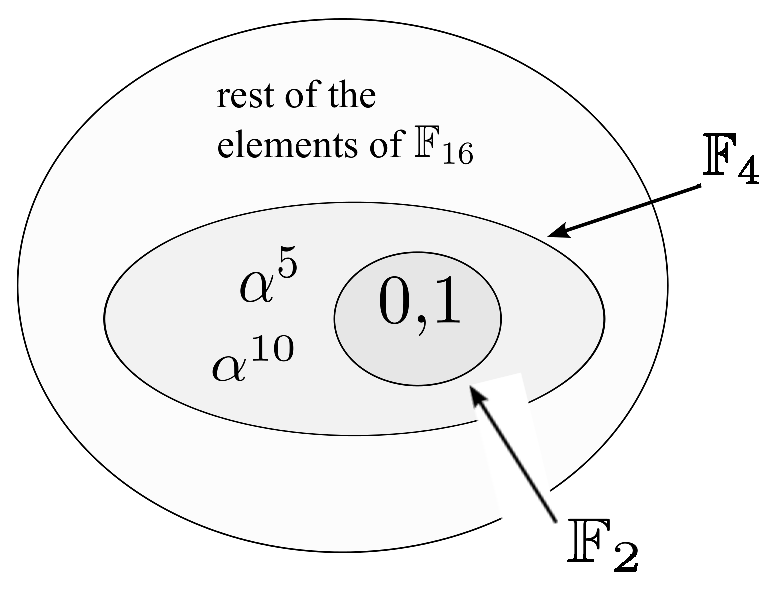
\includegraphics[scale=0.7]{./figures/field-cont}
\end{center}
\caption{Containment of Fields: $\F_2 \subset \F_4 \subset \F_{16}$}
\label{fig:contain2_4_16}
\end{figure}

Consider the element $\alpha^5$ of $\F_{16}$. 
Deriving all $(\alpha^5)^i$ for $i \geq 0$ 
over $\F_{16}$ gives the following recurrence:
\begin{eqnarray}
(\alpha^5)^0&=&1\nonumber \\
(\alpha^5)^1 &=& \alpha^5\nonumber \\
(\alpha^5)^2 &=& \alpha^{10}\nonumber \\
(\alpha^5)^3 &=& \alpha^{15} = 1
\end{eqnarray}
The only elements that are generated in this recurrence are $\{1,\alpha^5,\alpha^{10}\}$.
Every field contains $\{0,1\}$, so the elements $\{0,1,\alpha^5,\alpha^{10}\}$ form $\F_4$.
Let $P(x)=x^4+x^3+1$ be the primitive polynomial used to generate
$\F_{2^4}=\F_{16}$. A primitive polynomial of degree $2$ used to generate $\F_{2^2}=\F_4$
can be found as follows:
\begin{eqnarray}
& &(x+\alpha^5)\cdot(x+\alpha^{10}) \mod P(x) \nonumber \\
&=& x^2+(\alpha^{10}+\alpha^5)x+\alpha^{15} \mod P(x) \nonumber \\
&=& x^2+x+1
\end{eqnarray}

\begin{Theorem}
$\F_{2^n}\subset\F_{2^m}$ iff $n \mid m$, i.e. if $n$ divides $m$.
\end{Theorem}

Therefore:
\begin{itemize}
\item $\F_2 \subset \F_{2^2} \subset \F_{2^4} \subset \F_{2^8} \subset \dots$
\item $\F_2 \subset \F_{2^3} \subset \F_{2^9} \subset \F_{2^{27}} \subset \dots$
\item $\F_2 \subset \F_{2^5} \subset \F_{2^{25}} \subset \F_{2^{125}} \subset \dots,$ and so on
\end{itemize}

\begin{Definition}
The {\bf algebraic closure} of the Galois field $\F_{2^k}$, denoted $\overline{\Fkk}$, is the 
union of all fields $\F_{2^n}$ such that $k \mid n$.
\end{Definition}


%%%%%%%%%%%%%%%%%%%%%%%%%%%%%%%%%%%%%%%%%%%%%%%%%%%%%%
\subsection{Polynomial Interpolation over Galois Fields}

In the construction of digital circuits, arbitrary mappings between 
two bit-vectors of size $k$ can be constructed. Each such
mapping generates a function $f: \B^k \rightarrow \B^k$.
As every $k$-bit vector can be construed as an element in $\Fkk$ 
(as shown in the previous section), 
every such function also corresponds to a function over a 
Galois field: $f: \Fkk \rightarrow \Fkk$. 

\begin{Definition}
A function $f: \mathbb{R} \rightarrow \mathbb{R}$ over a ring $R$ is 
considered a {\bf polynomial function} if there exists a polynomial
$\Func \in \mathbb{R}[x_1,\dots,x_d]$ such that 
$\Func(x_1,\dots,x_d) = f(x_1,\dots,x_d)$.
\end{Definition}

\begin{Theorem}
From \cite{ff:1997}: 
Let $\Fq$ be a Galois field of $q$ elements where $q$ is a power of a
prime integer. Given any function $f: \Fq \to \Fq$, there exists a 
polynomial 
$\Func \in \Fq [x]$ such that $f(a) = \Func(a)$, for all $a \in \Fq$.
Thus, every function $f: \Fq \to \Fq$ is a polynomial function.
\end{Theorem}

Thus, since every function over a Galois field, $f: \Fkk \rightarrow \Fkk$, 
is a polynomial function, 
every mapping between two bit-vectors of size $k$ 
is a polynomial function over $\Fkk$.
Furthermore, every polynomial can be derived using Lagrange interpolation.

\begin{Theorem} ({\bf Lagrange Interpolation}): \\
Given a set of $k$ data points over a function $f$,
\begin{equation}
(x_0,f(x_0)),\dots,(x_{k-1},f(x_{k-1})) \nonumber
\end{equation}
where no two $x_i \in \{x_0,\dots,x_{k-1}\}$ are the same elements,
the polynomial representation of $f$, $\Func(x)$, can be interpolated as 
follows:  
\begin{eqnarray}
\Func(x) = \sum_{i=0}^{k-1} f(x_i)\cdot L_i(x) \nonumber \\
L_i(x) =  \prod_{(0\leq j \leq k-1),(j\neq i)}\frac{x-x_j}{x_i-x_j} \nonumber  
\end{eqnarray}
\end{Theorem}

By applying Lagrange interpolation over every element in the Galois
field $\Fkk$, 
we can derive the polynomial representation $\Func$ of any function 
$f:\Fkk \rightarrow \Fkk$. Furthermore, $\Func$ is a polynomial of degree 
at most $2^k-1$ in $x$ and $\Func(a)=f(a)$ for all $a \in \Fkk$.

While every function over a Galois field is a polynomial function,
not every function over the integer ring $\mathbb{Z}$ is a polynomial 
function.


%\begin{equation}
%\Func(x) = \sum_{k=1} ^q  \frac{ \prod_{i \neq k}  (x -x_i)}{\prod_{i \neq k}(x_k -x_i)} \cdot \f(x_k)
%\label{eqn:lagrange}
%\end{equation}

%As every function over a Galois field is also a polynomial 
%function, any mapping between two $k$-bit vectors is also a 
%polynomial function when analyzed over $\Fkk$.

%By analyzing $\Func$ over each point in $\Fq$ and applying 
%{\bf Lagrange's interpolation formula}, shown in 
%Equation \ref{eqn:lagrange}, one can interpolate the 
%polynomial representation, $f_p$, of the function $\Func$.

%Then, $f_p$ is a polynomial of degree at most $q-1$ in $x$ and
%$f_p = \F(a)$ for all $a \in \Fq$, and $\F(x)$.
%Thus, $f_p$ is a polynomial function representation of $\Func$. 


\begin{Example} {\it
Let $A = \{a_2, a_1, a_0\}$ and $Z = \{z_2,z_1,z_0\}$ be 3-bit vectors.
Thus, $A$ and $Z \in \mathbb{B}^3$. 
Consider the following function:
\begin{equation}
f:Z[2:0] = A[2:0]>>1 \nonumber
\end{equation}
$f$ is a {\bf bit-vector right shift} operation on $A$. 
This function can be analyzed as a mapping over different forms: 
$\mathbb{B}^3 \rightarrow \mathbb{B}^3$,
$\mathbb{Z}_8 \rightarrow \mathbb{Z}_8$, and
$\F_{2^3} \rightarrow \F_{2^3}$. These mappings from $A$ to $Z$ 
are:

\begin{center}
{\small
\begin{tabular}{c|c|ccc|c|c|} 
$\{a_2a_1a_0\}\in\mathbb{B}^3$  & $A\in \mathbb{Z}_8$ & $A\in \F_{2^3}$ &$\rightarrow$& $\{z_2z_1z_0\}\in\mathbb{B}^3$ &$Z\in \mathbb{Z}_8$ & $Z\in \F_{2^3}$ \\
\hline
000  &0&0 &$\rightarrow$&000 &0& 0 \\
001  &1&1 &$\rightarrow$&000 &0& 0 \\
010  &2&$\alpha$ & $\rightarrow$ & 001&1& 1 \\
011  &3&$\alpha + 1$ &$\rightarrow$& 001&1 &1 \\
100  &4&$\alpha^2$ &$\rightarrow$& 010 &2&  $\alpha$ \\
101  &5&$\alpha^2 + 1$ &$\rightarrow$&010 &2& $\alpha$ \\
110  &6&$\alpha^2 + \alpha$&$\rightarrow$& 011 &3&$\alpha + 1$ \\
111  &7&$\alpha^2 + \alpha + 1$ &$\rightarrow$& 011 &3&$\alpha + 1$\\
\hline
\end {tabular}
}
\end{center}

$f: \mathbb{Z}_8 \rightarrow \mathbb{Z}_8$ is not a polynomial function 
(this can be verified using the results of \cite{singmaster}
\cite{chen_95} \cite{chen_96}). However, $f: \F_{2^3} \rightarrow \F_{2^3}$
is a polynomial function.
By applying Lagrange's interpolation formula to $f$ over $\F_{2^3}$ for 
every element in $\F_{2^3}$, 
we obtain the following polynomial function: $Z =
(\alpha^2+1)A^4+(\alpha^2+1)A^2$, where $P(\alpha) = \alpha^3 +
\alpha + 1 = 0$. 
}
\end{Example}

Since every function over $\Fkk$ is a polynomial function, the 
functional mapping of a Galois field arithmetic circuit over
$\Fkk$ must exist in polynomial form. 
Construction of these arithmetic circuits is described next.


%%%%%%%%%%%%%%%%%%%%%%%%%%%%%%%%%%%%%%%%%%%%%%%%
%%%%%%%%%%%%%%%%%%%%%%%%%%%%%%%%%%%%%%%%%%%%%%%%
%%%%%%%%%%%%%%%%%%%%%%%%%%%%%%%%%%%%%%%%%%%%%%%%
\section{Hardware Implementations of Arithmetic Operations Over Galois Fields}

There are two main applications of hardware implementations of Galois field 
arithmetic.
In the first case, Galois field arithmetic computations, such as {\sc add or mul},  
are implemented in hardware, and  
algorithms are then implemented in software 
(e.g. cryptoprocessors \cite{ST23} \cite{kobayashi}). 
In other cases, the entire design can be implemented in hardware, such as a one-shot 
Reed-Solomon encoder-decoder chip \cite{reed-solo-chip} \cite{ecc163}, or point 
multiplication circuitry \cite{ecc:software} used in elliptic curve cryptosystems. 
Therefore, there has been extensive research in efficient hardware design of 
primitive arithmetic computations over Galois fields.
In this section, we describe the design principles of such circuits with focus 
on their architecture and verification complexity.

{\bf Addition} in $\Fkk$ is performed by correspondingly adding the
polynomials together and reducing the coefficients of the result modulo $2$.
\begin{Example}
Given $A=\alpha^3+\alpha^2+1=(1101) $ and $B=\alpha^2+1=(0101)$ in $\mathbb{F}_{2^4}$, 
\begin{equation}
A+B=(\alpha^3+\alpha^2+1)+(\alpha^2+1)=(\alpha^3) + (\alpha^2+\alpha^2) +(1+1)=\alpha^3=(1000). \nonumber
 \end{equation}
\end{Example}

Effectively, the addition operation is only performed on the coefficients, 
which are in $\F_2$. 
As addition over $\F_2$ performs an {\it XOR} operation,
constructing an addition circuit over $\Fkk$ is trivial as it
only consists of $k$ number of {\it XOR} gates. 
A $4$-bit adder over $\F_{2^4}$ is shown in
Fig. \ref{fig:adder4}.
\begin{figure}[H]
\begin{center}
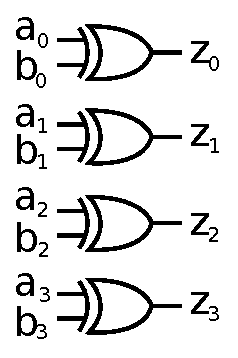
\includegraphics[scale=0.6]{figures/adder4bit}
\end{center}
\caption{$4$-bit adder over $\mathbb{F}_{2^4}$.}
\label{fig:adder4}
\end{figure}

{\bf Multiplication} $Z =A\times B \pmod{ P(x) }$ in $\Fkk$ conceptually consists of 
two steps.
In the first step, the multiplication $A\times B$ is performed. In the second 
step, the result is reduced
modulo the irreducible polynomial $P(x)$.
This multiplication procedure is shown in Example \ref{exp:mul}.

%\ref{exp1}, 
\begin{Example}
\label{exp:mul}
Consider the field $\mathbb{F}_{2^4}$ with the irreducible polynomial 
$P(x)=x^4+x^3+1$ and $P(\alpha)=0$. We take as inputs:
$A=a_0+a_1\cdot \alpha+a_2\cdot \alpha^2+a_3\cdot \alpha^3$ and
$B=b_0+b_1\cdot \alpha+b_2\cdot \alpha^2+b_3\cdot \alpha^3$. 
We have to perform the multiplication $Z =A\times B \pmod{ P(x) }$. The coefficients
of $A = \{a_0, \dots, a_3\}, B = \{b_0, \dots, b_3\}$ are in
$\mathbb{F}_2 = \{0, 1\}$. This multiplication can be performed as
shown:

{\begin{tabular}{c c c c c c c c}
  &   &   & $a_3$ & $a_2$ & $a_1$ & $a_0$  \\ 
 $\times$&   &   & $b_3$ & $b_2$ & $b_1$ & $b_0$  \\ 
 \hline
 &   &   & $a_3\cdot b_0$ & $a_2 \cdot b_0$ & $a_1\cdot b_0$ & $a_0\cdot b_0$ \\
 &  & $a_3\cdot b_1$ & $a_2\cdot b_1$ & $a_1 \cdot b_1$ & $a_0\cdot b_1$ &   \\
 & $a_3\cdot b_2$ & $a_2\cdot b_2$ & $a_1\cdot b_2$ & $a_0\cdot b_2$ &  &   \\
 $a_3\cdot b_3$ & $a_2\cdot b_3$ & $a_1\cdot b_3$ & $a_0\cdot b_3$ &  &  &   \\
 \hline
 $s_6$& $s_5$  & $s_4$  & $s_3$ & $s_2$  & $s_1$   & $s_0$ 
\end{tabular}}

The result $Sum = s_0+s_1\cdot \alpha + s_2\cdot \alpha^2 + s_3\cdot
\alpha^3 + s_4\cdot \alpha^4 + s_5\cdot \alpha^5 + s_6\cdot \alpha^6$,
where
\begin{eqnarray}
	s_0  &=&  a_0\cdot b_0 \nonumber \\ 
	s_1  &=&  a_0\cdot b_1 + a_1\cdot b_0 \nonumber \\
	s_2  &=&  a_0\cdot b_2 + a_1\cdot b_1 + a_2\cdot b_0 \nonumber \\
	s_3  &=&  a_0\cdot b_3 + a_1\cdot b_2 + a_2\cdot b_2 +  a_3\cdot b_1\nonumber \\
	s_4  &=&  a_1\cdot  b_3 + a_2\cdot b_1 + a_3\cdot b_1 \nonumber \\
	s_5  &=&  a_2\cdot b_3 + a_3\cdot b_2  \nonumber \\
	s_6  &=&  a_3\cdot b_3   \nonumber
\end{eqnarray}
 Here the multiply ``$\cdot$'' and add ``$+$'' operations are performed
modulo 2, so they can be implemented in a circuit using AND and XOR
gates respectively. Note that unlike integer multipliers, there are no carry-chains
in the design, as the coefficients are always reduced modulo $2$. 
However, the result is yet to be reduced modulo the primitive
polynomial $P(x) = x^4 + x^3 + 1$. This transforms every exponent representation, 
$\alpha^d$, to a polynomial representation where $d\geq k=4$.

{\begin{tabular}{|c c c c | l }
 \multicolumn{5}{c}{} \\
 \multicolumn{1}{c}{$\alpha^3$} & $\alpha^2$ & $\alpha$ & \multicolumn{1}{c}{$1$} &  \\
\hhline{----~}
  $s_3$ 	&$s_2$  	&$s_1$   &$s_0$ 	&   \\
 \hline
 $s_4$ 		&$0$		&$0$ 	 &$s_4$  	&$s_4\cdot \alpha^4 \pmod{P(\alpha)} = s_4 \cdot (\alpha^3 + 1)$\\
 $s_5$ 		&$0$		&$s_5$   &$s_5$     &$s_5\cdot \alpha^5 \pmod{P(\alpha)} = s_5\cdot (\alpha^3+ \alpha + 1)$\\
 $s_6$ 		&$s_6$		&$s_6$   &$s_6$     &$s_6\cdot \alpha^6 \pmod{ P(\alpha)} = s_6\cdot( \alpha^3 + \alpha^2 + \alpha + 1)$\\
 \hline
 $z_3$ 		&$z_2$ 		&$z_1$   &$z_0$ 	&\\
 \multicolumn{5}{c}{} \\
 \end{tabular}\par}

The final result (output) of the circuit is: $Z = z_0 + z_1 \alpha + z_2
\alpha^2 + z_3 \alpha^3$; where  $z_0=s_0+s_4+s_5+s_6; ~~z_1=s_1+s_5+s_6;
~~z_2=s_2+s_6; ~~z_3=s_3+s_4+s_5+s_6$. 
\end{Example}

%%%%%%%%%%%%%%%%%%%%%%%%%%%%%%%%%%%%%%%%%%%%%%%%%%%%%%%%%%%

The above multiplier design is called the {\it Mastrovito multiplier} \cite{mastro:1989} 
which is the most straightforward way to design a multiplier over $\mathbb{F}_{2^k}$. 
A logic circuit for a $4$-bit {\it Mastrovito} multiplier over {\it Galois field} $\mathbb{F}_{2^4}$ is illustrated in Fig. \ref{fig:mas4}.

\begin{figure}[H]
	\begin{center}
	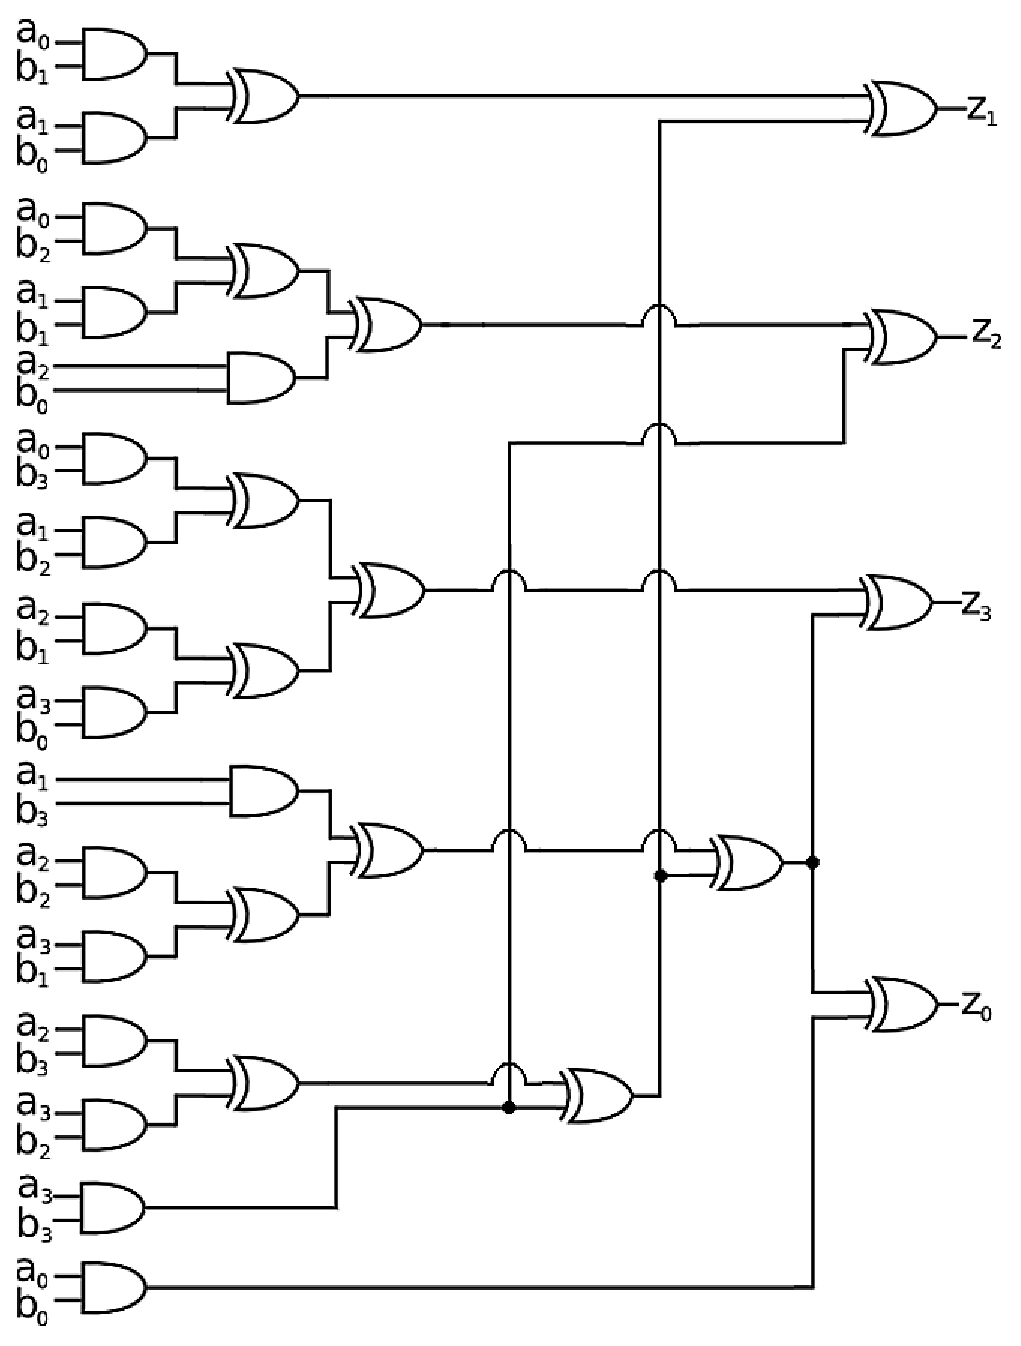
\includegraphics[scale=0.60]{figures/mul4bit.eps}
	\end{center}
	\caption{Mastrovito multiplier over $\mathbb{F}_{2^4}$.}
	\label{fig:mas4}
\end{figure}

Modular multiplication is at the heart of many public-key cryptosystems, 
such as Elliptic Curve Cryptography (ECC) \cite{ecc:1986}. 
Due to the very large field size (and hence the data-path width) used in these cryptosystems, 
the above {\it Mastrovito} multiplier architecture is inefficient, especially when 
exponentiation and repeat multiplications are performed.
Therefore, efficient hardware and software implementations of modular multiplication 
algorithms are used to overcome the complexity of such operations. 
One such algorithm which we will focus on is the Montgomery reduction \cite{PT:1985} \cite{acar:1998}.

\subsection{Montgomery Multipliers}
Montgomery Reduction (MR) computes: 

\begin{equation}
G=MR(A,B)=A\cdot B \cdot R^{-1} \pmod {P(x)}
\end{equation}
where $A,B$ are $k$-bit inputs, $R={\alpha}^k$, $R^{-1}$ is multiplicative
inverse of $R$ in $\mathbb{F}_{2^k}$, and $P(x)$ is the irreducible polynomial for
$\mathbb{F}_{2^k}$. Since Montgomery reduction cannot directly compute $A\cdot B$, 
we need to pre-compute $A\cdot R$ and $B\cdot R$,
as shown in Fig. \ref{fig:mm4}.  

\begin{figure}[h]
	\begin{center}
	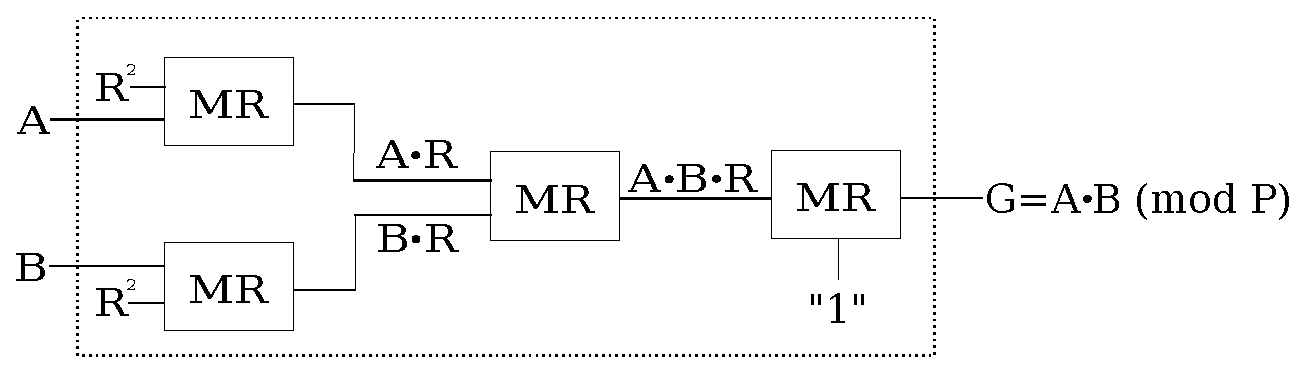
\includegraphics[scale=0.50]{figures/mmcircuit}
	\end{center}
	\caption{Montgomery multiplier over $\mathbb{F}_{2^k}$}
	\label{fig:mm4}
\end{figure}

Each $\it MR$ block in Fig. \ref{fig:mm4} represents a Montgomery reduction step 
which is a hardware implementation of the algorithm shown in 
Algorithm \ref{alg:mont}. 

\begin{algorithm}
\SetAlgoNoLine

 \KwIn{$A(x), B(x)\in \mathbb{F}_{2^k}$; irreducible polynomial $P(x)$.}
 \KwOut{$G(x)=A(x)\cdot B(x)\cdot x^{-k} \pmod {P(x)}$.}
%%%%%%%%%%%%%%%%%%%%
  $G(x):=$0 \\
  \For { ($i=0$;   $i \le k-1$; ++i ) }
  {
	$G(x):=G(x)+A_i\cdot B(x)$ \CommentSty{/*$A_{i}$ is the $i^{th}$ bit of $A$*/\;}
	$G(x):=G(x)+G_0\cdot P(x)$ \CommentSty{/*$G_{0}$ is the lowest bit of $G$*/\;}
	$G(x):=G(x) / x$ \CommentSty{/*Right shift $1$ bit*/\;}
  }
\caption{Montgomery Reduction Algorithm \cite{acar:1998}}\label{alg:mont}
\end{algorithm}

The design of Fig. \ref{fig:mm4} is not efficient to computing
$A\cdot B \pmod{ P(x)}$ when compared to the Mastrovito implementation.
However, when these multiplications are
performed repeatedly, such as in iterative squaring, then the
Montgomery approach speeds-up the computation. 
As shown in \cite{wu:2002}, the critical path delay and gate counts of a squarer 
designed using the Montgomery approach are much smaller than the traditional 
approaches.

\subsection{Circuit Designs over Composite Fields}
The Galois field $\mathbb{F}_{2^k}$ is a $k$-dimensional vector space over the
sub-field $\mathbb{F}_2$. If $k = m\cdot n$, the field $\mathbb{F}_{2^k}$
can be decomposed as $\mathbb{F}_{(2^m)^n}$. Such a field representation is
called a {\bf composite field}, and it is constructed as a $n$-dimensional 
extension of the sub-field $\mathbb{F}_{2^m}$. The sub-field $\mathbb{F}_{2^m}$ is
called the ground field. Note that we have $\mathbb{F}_2 \subset \mathbb{F}_{2^m}
\subset \mathbb{F}_{(2^m)^n}$.

A Galois field arithmetic circuit over $\Fkk$ can thus be composed
as circuit over $\F_{(2^m)^n}$ if $k=m\cdot n$.
Since the base field is $\F_{2^m}$, this composite field circuit is
composed of blocks of $m$-bit multipliers and adders, along with 
$m$-bit buses that act as the inputs and outputs of these blocks.
A $\F_{2^4}$ Galois field multiplier designed over the composite field $\F_{(2^2)^2}$ is shown in 
Fig. \ref{fig:comp4exPrelim}.
Design methodologies of these circuits are examined more closely in Chapter \ref{ch:generalize}.

\begin{figure}[t]
        \centering
        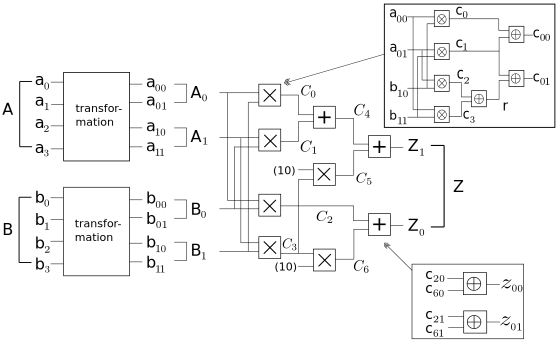
\includegraphics[width=.9\linewidth]{./figures/compMineSmall}
        \caption{$4$-bit composite multiplier designed over $\F_{(2^2)^2}$}\label{fig:comp4exPrelim}
\end{figure}

%% According to Theorem \ref{the:unique}, there exists an unique field of size $p^{k}$. 
%% This implies that $\mathbb{F}_{2^k}$ is isomorphic to
%% $\mathbb{F}_{(2^m)^n}$ when $k = m\cdot n$, and due to this isomorphism,
%% it is possible to derive one field representation from the other. 
%% The principle of constructing a composite field is described in \cite{phdpaar:1994}. 
%% We derive concrete steps for constructing circuits over composite fields.

%% To construct $\mathbb{F}_{(2^m)^n}$, we require a primitive polynomial of 
%% degree $n$, with coefficients from the ground field $\mathbb{F}_{2^m}$. 
%% Let $k=m\cdot n$. Given $\mathbb{F}_{2^k}$ and its primitive polynomial $P(x)$
%% of degree k, 
%% the primitive polynomial of the composite field can be easily
%% derived. We use the following notation:

%% \begin{itemize}
%% \item Let $P(x)$ denote the given primitive polynomial of general
%%   field $\mathbb{F}_{2^k}$. Let $\alpha$ be a root of the 
%%   this polynomial, i.e. $P(\alpha)=0$.  
%% \item Let $Q(x)$ denote the primitive polynomial of ground field
%%   $\mathbb{F}_{2^m}$. Let $\beta$ be a root of $\mathbb{F}_{2^m}$,
%%   i.e. $Q(\beta)=0$. Note that $Q(x)$ is a degree $m$ primitive
%%   polynomial over $\mathbb{F}_{2}$ so it is also known. 
%% \item Let $R(x)$ denote the primitive polynomial of composite field
%%   $\mathbb{F}_{(2^m)^n}$. Let $\gamma$ be a root,
%%   i.e. $R(\gamma)=0$. This polynomial $R(x)$ has to be derived. 
%% \end{itemize}

%% %To construct $R(x)$, we hae the following result 
%% \begin{Lemma}
%% From \cite{cf:2003}: Let $\mathbb{F}_{2^k}$ be decomposed as $\mathbb{F}_{(2^m)^n}$
%% where $k = m\cdot n$. Let $\gamma$ be the primitive root of the field $\mathbb{F}_{(2^m)^n}$. 
%% Then 
%% \begin{equation}
%% R(x)=\prod_{i=0}^{i=n-1}(x_i+\gamma^{2^{m \cdot i}})
%% \end{equation}
%% \end{Lemma}

%% Since $\mathbb{F}_{2^k}$ is isomorphic to $\mathbb{F}_{(2^m)^n}$, $\alpha$ and
%% $\gamma$ are the same elements ($\alpha=\gamma$).
%% Consider the representation of an element $A$ in $\mathbb{F}_{2^k}$ and its corresponding
%% representation in the composite field.

%% \begin{itemize}
%% \item Any element $A \in \mathbb{F}_{2^k}$ is represented as:
%% \begin{equation}
%% A=\sum_{i=0}^{i=k-1}a_i \cdot \alpha^i, a_i \in \mathbb{F}_{2}, \text{and}\	 P(\alpha) = 0
%% \end{equation}
%% \item The same element $A \in \mathbb{F}_{(2^m)^n}$ is represented as:
%% \begin{equation}
%% A=\sum_{i=0}^{i=n-1}A_i \cdot \gamma^i, A_i \in \mathbb{F}_{2^m}, \text{and} \	 R(\gamma) = 0
%% \end{equation}
%% \item The element $A_i$ needs to be represented in the ground field $\mathbb{F}_{2^m}$:
%% \begin{equation}
%% A_i=\sum_{j=0}^{j=m-1}a_{ij} \cdot \beta^j, a_{ij} \in \mathbb{F}_{2}, \text{and} \	 Q(\beta) = 0
%% \end{equation}
%% \end{itemize}

%% Thus, we need to find the relationship between the primitive roots
%% $\alpha$ and $\beta$ (or between $\gamma$ and $\beta$, since $\alpha =\gamma$), 
%% so as to be able to map the elements from $\mathbb{F}_{2^k}$ to $\mathbb{F}_{(2^m)^n}$. 
%% We use the following result \cite{cf:2003}:

%% \begin{Theorem}\label{thm:gamma}
%% For $\gamma \in \mathbb{F}_{(2^m)^n}$, and $\beta=\gamma^{\omega}$, where $\omega=(2
%% ^{m \cdot n}-1)/(2^m-1)$, then we have $\beta \in \mathbb{F}_{2^m}$. In other
%% words: 
%% \begin{equation}
%% \beta=\alpha^{(2^{m \cdot n}-1)/(2^m-1)}=\gamma^{(2^{m \cdot n}-1)/(2^m-1)} \label{eqn:relation}
%% \end{equation}

%% \end{Theorem}

%% The above result states the following: Since $\gamma$ is a primitive
%% root, it can be used to generate all the non-zero elements of $\mathbb{F}_{(2^m)^n}$. 
%% Moreover, $\beta$ is a primitive root of the ground field $\mathbb{F}_{2^m}$, 
%% which is a sub-field of $\mathbb{F}_{(2^m)^n}$ ( i.e. $\mathbb{F}_{2^m}
%% \subset \mathbb{F}_{(2^m)^n}$); so $\beta \in \mathbb{F}_{(2^m)^n}$. Therefore
%% an exponent of $\gamma$ can be used to generate $\beta$ as
%% $\beta=\gamma^{\omega}$, where $\omega$ is given in Theorem
%% \ref{thm:gamma}. Now that we have all the relationships between $\alpha,
%% \beta, \gamma$, it is possible to perform the decomposition. 

%% \begin{Example}
%% Consider the field $\mathbb{F}_{2^4}$ 
%% with $P(x) = x^4 + x^3 + 1$ and $P(\alpha)=0$.
%% In order to decompose it as $\mathbb{F}_{(2^2)^2}$,
%% perform the following steps:

%% \begin{enumerate}
%% \item 
%% Derivation of $R(x)$:
%% \begin{eqnarray}
%% R(x)&=&\prod_{i=0}^{i=1}(x+\gamma^{2^{2 \cdot i}}) \nonumber \\
%% &=&(x+\gamma)\cdot (x+\gamma^{2^2})               \nonumber \\
%% &=&x^2+(\gamma^4+\gamma) \cdot x+\gamma^5          
%% \end{eqnarray}
%% Notice that $R(\gamma) = \gamma^2 + (\gamma^4+\gamma) \cdot \gamma+\gamma^5 =0$.
%% \item 
%% Representation of element $A \in \mathbb{F}_{(2^2)^2}$:
%% \begin{eqnarray}
%% A& = & \sum_{i=0}^{i=1}A_i \cdot \gamma^i, A_i \in \mathbb{F}_{2^2}\nonumber \\
%%  & = & A_0 +A_1 \cdot \gamma
%% \end{eqnarray}
%% \item 
%% Representation of $A_0, A_1$ in $\mathbb{F}_{2^m}$:
%% \begin{eqnarray}
%% A_0=a_{00}+a_{01} \cdot \beta \nonumber \\
%% A_1=a_{10}+a_{11} \cdot \beta
%% \end{eqnarray}
%% where $a_{ij}\in \mathbb{F}_2$. $Q(x)$ can be any degree $m=2$ primitive
%% polynomial in the ground field  $\mathbb{F}_{2^2}$. For the sake of
%% this example, let $Q(x)=x^2+x+1$. 
%% \item Substitute $A_0, A_1$ into $A$:
%% \begin{eqnarray}
%% A&=&\sum_{i=0}^{i=1}(\sum_{j=0}^{j=1}a_{ij} \cdot \beta^j) \cdot \gamma^i \nonumber \\
%% &=&a_{00}+a_{01}\cdot \beta+(a_{10}+a_{11}\cdot \beta)\cdot \gamma   \end{eqnarray}
%% where each $a_{ij} \in \mathbb{F}_2$. From Equation (\ref{eqn:relation}), 
%% $\beta=\alpha^5=\gamma^5$. Substitute $\beta$ and
%% $\gamma$ with $\alpha$ to obtain:
%% \begin{eqnarray}
%% A&=&\sum_{i=0}^{i=1}(\sum_{j=0}^{j=1}a_{ij} \cdot \beta^j) \cdot \gamma^i \nonumber \\
%% &=&a_{00}+a_{01}\cdot \alpha^5+(a_{10}+a_{11}\cdot \alpha^5)\cdot \alpha \nonumber 
%% \end{eqnarray} 
%% Since $P(x)=x^4+x^3+1$ with $P(\alpha)=0$, then
%% \begin{equation}\label{a}
%% A \pmod {P(\alpha)}=a_{00}+a_{01}+a_{11}+(a_{01}+a_{10}+a_{11})\cdot \alpha+a_{1
%% 1} \cdot \alpha^2+(a_{01}+a_{11})\cdot \alpha^3
%% \end{equation}

%% \item The same element $A \in \mathbb{F}_{2^4}$ is represented as:
%% \begin{equation}\label{aa}
%% A=a_0+a_1\cdot \alpha+a_2\cdot \alpha^2+a_3\cdot \alpha^3 
%% \end{equation}

%% \item Since Eqns. \ref{a} and \ref{aa} represent the same element, we
%%   can match the coefficients of the the polynomials to obtain:
%% \begin{eqnarray}
%% a_0&=&a_{00}+a_{01}+a_{11} \nonumber \\
%% a_1&=&a_{01}+a_{10}+a_{11} \nonumber \\
%% a_2&=&a_{11} \nonumber \\
%% a_3&=&a_{01}+a_{11} \nonumber
%% \end{eqnarray}

%% This mapping can also be reversed and represented as a matrix $T$:
%% \begin{center}
%% $\begin{bmatrix} a_{00}\\ a_{01} \\a_{10} \\ a_{11}\end{bmatrix}
%% =
%% \begin{bmatrix} 1 & 0 & 0 & 1\\ 0 & 0 & 1 & 1\\ 0 & 1 & 0 & 1\\ 0 & 0
%%   & 1 & 0 \end{bmatrix} 
%% \begin{bmatrix} a_0\\ a_1 \\a_2 \\ a_3\end{bmatrix}$
%% \end{center}
%% \end{enumerate}

%% Now we have successfully derived the composite field representation
%% $\mathbb{F}_{(2^2)^2}$ from $\mathbb{F}_{2^4}$. The element $A \in \mathbb{F}_{2^4}$ is
%% represented as $A = a_0 + a_1 \alpha + a_2 \alpha^2 + a_3 \alpha^3$,
%% where $P(\alpha) = 0$. The same element $A$ is represented in $\mathbb{F}_{(2^2)^2}$ as:
%% \begin{eqnarray}
%% A&=&A_0+A_1 \cdot \alpha \nonumber \\
%% A_0&=&a_{00}+a_{01} \cdot \alpha^5 \nonumber \\
%% A_1&=&a_{10}+a_{11} \cdot \alpha^5 \nonumber \\
%% a_{00}&=&a_0+a_3 \nonumber \\
%% a_{01}&=&a_2+a_3 \nonumber \\
%% a_{10}&=&a_1+a_3 \nonumber \\
%% a_{11}&=&a_2 \nonumber 
%% \end{eqnarray}

%% In the above equations, $\alpha = \gamma$ and $R(\gamma) = 0$. 
%% \end{Example}

%% A Galois field multiplier circuit over $\Fkk$ can thus be composed
%% as multiplier over $\F_{(2^m)^n}$ if $k=m\cdot n$.
%% Since the base field is $\F_{2^m}$, this composite field circuit is
%% composed of blocks of $m$-bit multipliers and adders, along with 
%% $m$-bit buses that act as the inputs and outputs of these blocks.

%% \begin{figure}[h!]
%% \centerline{
%% 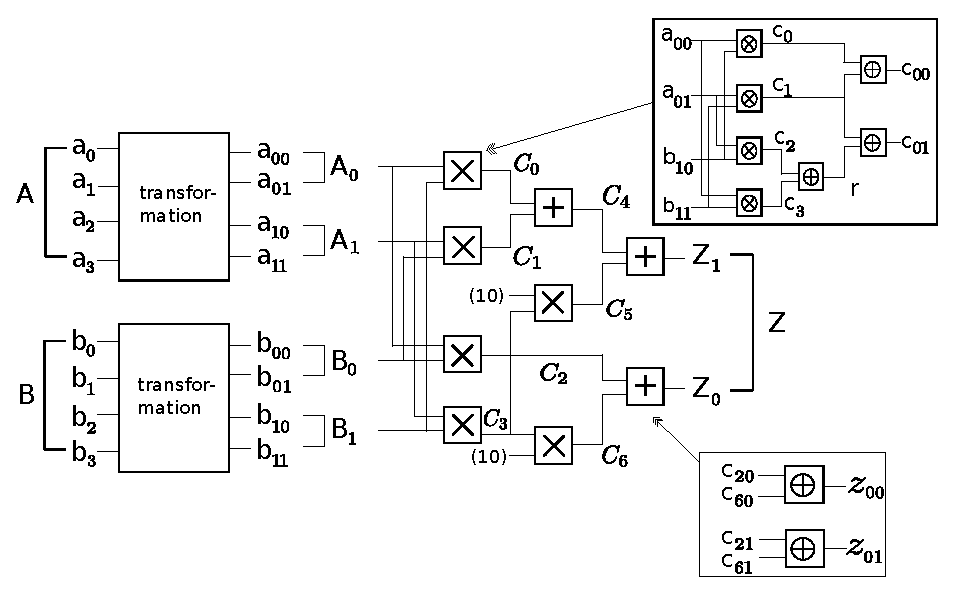
\includegraphics[width=\linewidth]{./figures/compMineSmall.eps}
%% }
%% \caption{Galois field multiplier over the composite field $\mathbb{F}_{(2^2)^2}$}
%% \label{fig:mas22}
%% \end{figure}

%% \begin{Example}
%% Consider the $4$-bit Mastrovito multiplier circuit over $\F_{2^4}$
%% shown in Figure \ref{fig:mas4}, where $A$ and $B$ are the $4$-bit 
%% word-level inputs and $\{a_0,a_1,a_2,a_3,b_0,b_1,b_2,b_3\}$ are
%% primary inputs, thus
%% \begin{eqnarray}
%% A=a_0+a_1\alpha+a_2\alpha^2+a_3\alpha^3 \nonumber \\
%% B=b_0+b_1\alpha+B_2\alpha^2+B_3\alpha^3 \nonumber
%% \end{eqnarray}

%% Since the field $\F_{2^4}$ can be decomposed as $\F_{(2^2)^2}$, 
%% this multiplier can be constructed as a composite field multiplier
%% over $\F_{(2^2)^2}$ with the base field $\F_{2^2}$.
%% Such a multiplier is shown Figure \ref{fig:mas22} and
%% is represented as follows:
%% \begin{eqnarray}
%% A = A_0+A_1\gamma \nonumber \\
%% B = B_0+B_1\gamma \nonumber \\
%% A_0=a_{00}+a_{01} \cdot \beta \nonumber \\
%% A_1=a_{10}+a_{11} \cdot \beta \nonumber \\
%% B_0=b_{00}+b_{01} \cdot \beta \nonumber \\
%% B_1=b_{10}+b_{11} \cdot \beta \nonumber
%% \end{eqnarray}
%% where $A_0,A_1,B_0,B_1$ are the $2$-bit inputs $\in \F_{2^2}$
%% composed of $a_{00},a_{01},a_{10},a_{11},b_{00},b_{01},b_{10},b_{11}$, 
%% which are the bit-level inputs to the composite field multiplier
%% derived from the transformation of $\{a_0,a_1,a_2,a_3,b_0,b_1,b_2,b_3\}$.
%% Correspondingly, each block in Figure \ref{fig:mas22}
%% internally represents a $2$-bit operation: $\times$ represents $2$-bit
%% {\it multiplication} and $+$ represents $2$-bit {\it addition} over
%% the ground field.
%% \end{Example}

%\afterpage{%
%    \clearpage% Flush earlier floats (otherwise order might not be correct)
%    \thispagestyle{empty}% empty page style (?)
%	\global\pdfpageattr\expandafter{\the\pdfpageattr/Rotate 90}
%    \begin{landscape}% Landscape page
     
%\begin{sidewaysfigure}
%\begin{figure}[h!]
%\centerline{
%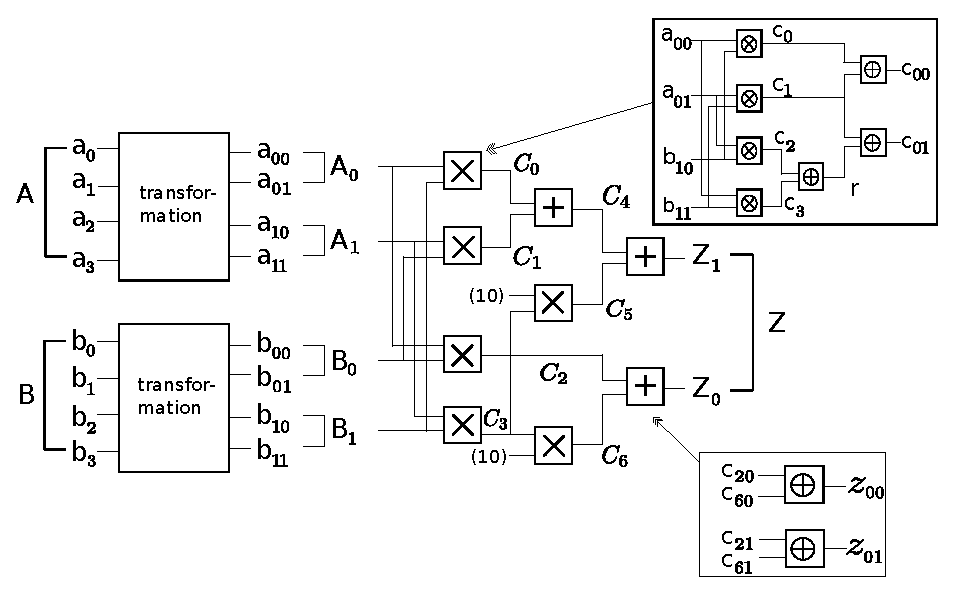
\includegraphics[width=.9\linewidth]{./figures/compMineSmall.eps}
%}
%\caption{Mastrovito multiplier over the composite field $\mathbb{F}_{(2^2)^2}$}
%\label{fig:mas22}
%\end{figure}
%\end{sidewaysfigure}
%  
%    \end{landscape}
%    \clearpage% Flush page
%	\global\pdfpageattr\expandafter{\the\pdfpageattr/Rotate 0}
%}

%%%%%%%%%%%%%%%%%%%%%%%%%%%%%%%%%%%%%%%%%%%
\subsection{Applications to Elliptic Curve Cryptography}
Elliptic Curve Cryptography (ECC) is one of the most influential applications 
of Galois fields.
ECC is an approach to public-key (or asymmetric-key) cryptography based on the 
algebraic structure of elliptic curves over Galois fields. Due to the complex 
nature of these curves, key sizes in ECC can be smaller than other public-key
cryptography techniques while providing the same level of security \cite{ecc:book}.
The main operations of encryption, decryption and authentication in ECC 
rely on {\it point multiplications}.


Point multiplication involves a series of addition and doubling of points on the 
elliptic curve.
A drawback of traditional point multiplication is that each point addition and 
doubling require a multiplicative inverse operation over Galois fields, 
the computation of which is costly.
Modern methods, however, represent the points in 
projective coordinate systems \cite{ecc:software},
which has eliminated the need for a multiplicative inverse operation by replacing it 
with addition and multiplication operations over Galois fields.
This has increased the efficiency of point multiplication operations, but it has also
increased the need for fast, custom hardware designs of Galois field arithmetic.

In-depth analysis of elliptic curve theory is beyond the scope of this 
dissertation. Instead, we will look at some examples of point addition and point doubling to
give a general idea of the operations involved in ECC and how they apply to Galois 
field arithmetic. Our experiments use custom Galois field arithmetic designs based 
on L$\acute{o}$pez-Dahab (LD) coordinate system \cite{eccld}, so these examples will
use the same coordinate system. 

\begin{figure}[h]
	\begin{center}
	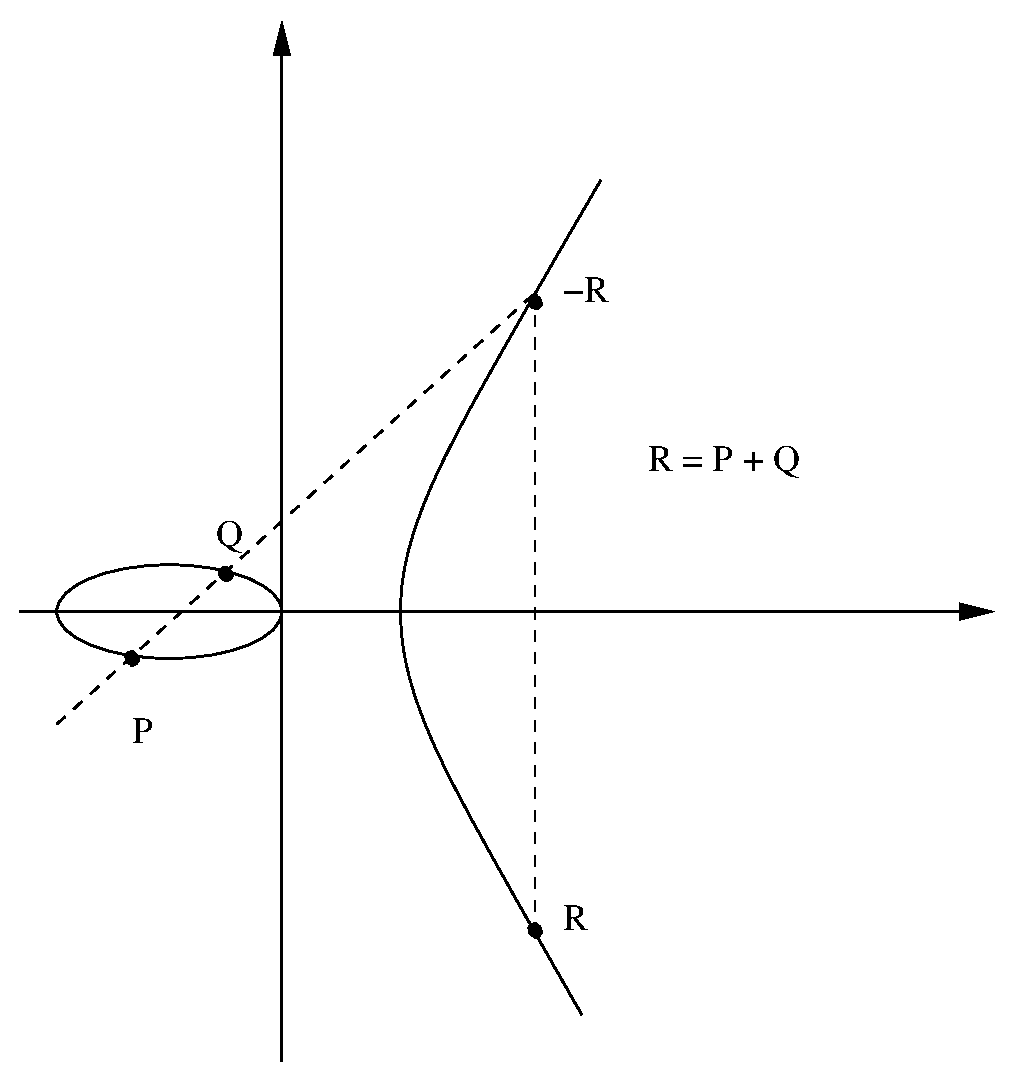
\includegraphics[scale=0.50]{figures/ecc}
	\end{center}
	\caption{Point addition over an Elliptic Curve (R=P+Q)}
	\label{fig:ecc}
\end{figure}

\begin{Example}
Consider point addition in a LD projective coordinate system, 
as seen in Fig. \ref{fig:ecc}. 

Given an elliptic curve: $Y^2 + XYZ = X^3Z + aX^2Z^2 + bZ^4$ over $\mathbb{F}_{2^k}$, 
where $X,Y,Z$ are $k$-bit vectors
that are elements in $\mathbb{F}_{2^k}$ and similarly, 
$a, b$ are constants from the field. 
Let $P + Q = R$ represent point addition over the elliptic curve.
$P=(X_1, Y_1, Z_1)$ and $Q=(X_2, Y_2, 1)$ are given.
Then $R=(X_3, Y_3, Z_3)$ can be computed as follows:

\begin{align*}
A &= Y_2 \cdot Z_1^2 + Y_1 \\
B &= X_2 \cdot Z_1 + X_1 \\
C &= Z_1 \cdot B \\
D &= B^2 \cdot(C + a Z_1^2) \\
Z_3 &= C^2 \\
E &= A \cdot C  \\
X_3 &= A^2 + D + E  \\
F &= X_3 + X_2 \cdot Z_3 \\
G &= X_3 + Y_2\cdot Z_3 \\
Y_3 &= E\cdot F + Z_3 \cdot G \\
\end{align*}
\end{Example}

\begin{Example}
Consider point doubling in a LD projective coordinate system. 
Given an elliptic curve: $Y^2 + XYZ = X^3Z + aX^2Z^2 + bZ^4$. 
Let 2($X_1$, $Y_1$, $Z_1$) = ($X_3$, $Y_3$, $Z_3$), then

\begin{align*}
X_3 &= X_1^4 + b \cdot Z_1^4  \\
Z_3 &= X_1^2 \cdot Z_1^2 \\
Y_3 &= b Z_1^4 \cdot Z_3 + X_3 \cdot (aZ_3 + Y_1^2 + bZ_1^4 ) \\
\end{align*}
\end{Example}

In the above examples, polynomial multiplication and squaring operations can be 
implemented in hardware using Montgomery reductions over Galois fields $\mathbb{F}_
{2^k}$. In practical applications, the field size $k$ of $\mathbb{F}_{2^k}$ is $163$,
or larger. However, there are no word-level 
abstraction techniques applicable to circuits of such size, so hardware 
implementations of Galois field arithmetic circuits 
cannot benefit from the many advantages of abstraction.
Thus, we propose a computer-algebra approach to word-level polynomial abstractions 
of Galois field arithmetic circuits.
Recent computer-algebra formal verification techniques \cite{lv:phd} 
have been able to verify these circuits up to $163$ bits. 
We propose an application of our abstraction approach to improve these techniques. 
These improvements allow us to perform formal verification of these
circuits up to $571$ bits. These proposals are described in detail in 
subsequent chapters.
